\section{Security}\label{sec:security}
    The Hashgraph is an \gls{abft} protocol tolerant to $\frac{n}{3}$ byzantine faults. The following section describes how this tolerance is kept when swapping nodes between the active and passive pool, and the incentive structure assuring security by using \textit{time-based staking}.

\subsection{Time-Based Staking}
    To join the Tagion Network through the passive pool, participants must stake a minimum fixed amount of \acrfull{tgn}. Staking refers to investing some amount of \gls{tgn} in the network for a predetermined amount of time\footnote{It is also possible to restake ones staked \gls{tgn} after this predetermined period ends. This, though, comes with the cost of losing some seniority (defined in a later section)}. This ensures node operators have a vested interest in the network, and also deters malicious actions since penalties can be enforced through slashing (reduction in staked \gls{tgn}). 
    The amount of \gls{tgn} staked, combined with ones seniority (defined later), determines ones chance of joining the active pool. This is contrast to being swapped out of the active pool, where the probability is uniform, and does not depend on your stake. This ensures that while nodes with more \gls{tgn} participate in the Hashgraph more frequently, their voting power remains neither stronger nor more enduring than nodes with fewer \gls{tgn}. This is contrast to most staking systems, where the amount of staked \gls{tgn} determines the weight of your vote. Tagion's staking guarantees that consensus isn't unduly skewed by stake magnitude, promoting a decision-making ethos that prioritises equality and fairness.

\subsection{Time and Amount}
    Your staked amount of \gls{tgn} fundamentally determines your chance of being selected as an active node. The probability of joining the active pool increases linearly with every \gls{tgn} staked. This method is preferred over a diminishing returns model. The latter could incentivise operators to launch several nodes, compromising network transparency by suggesting the system is more decentralised than it truly is. To foster enduring commitment among node operators and promote long-term stability within the network, Tagion utilises seniority. Those who maintain their stakes for prolonged periods, while continuously operating a node supporting the network throughout, are granted heightened seniority. This seniority enhances the probability of joining the active pool.
    
    \begin{figure}[H]
	   \centering
	   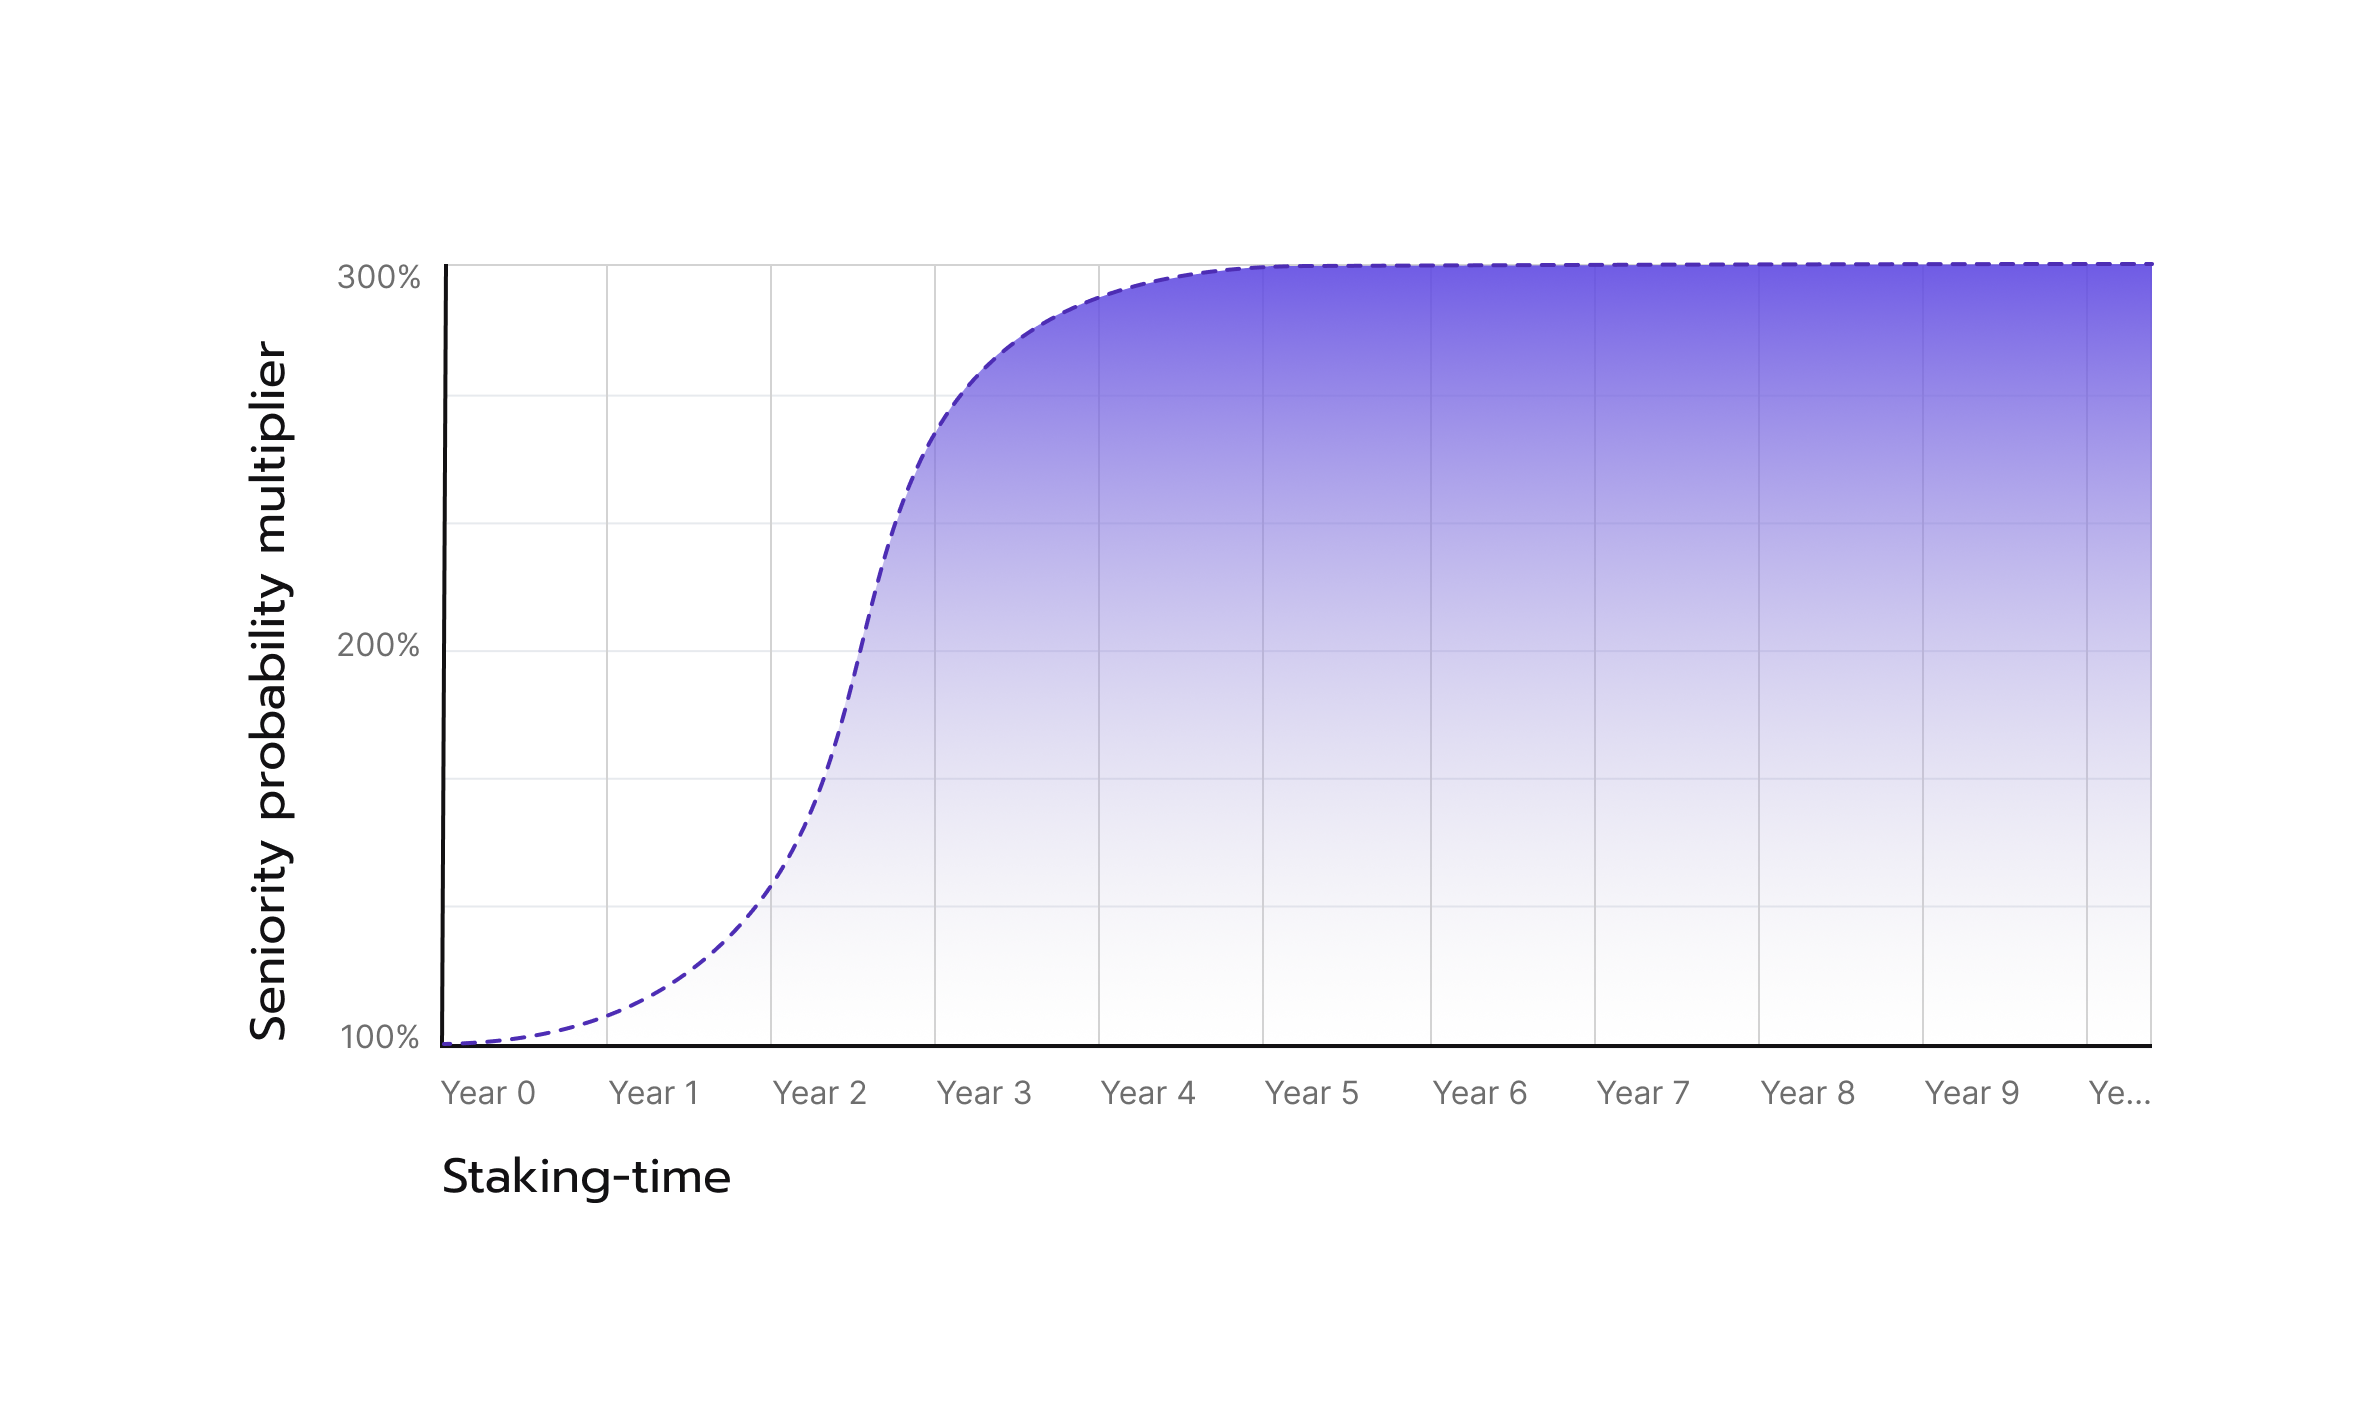
\includegraphics[width=1\textwidth]{figures/seniority.png}
	   \caption{How seniority affects the probability of becoming an active node}
	   \label{figure:seniority}
    \end{figure}
    
    The seniority probability multiplier follows an increasing S-curve. Initially, the probability of joining the active pool is purely determined by the amount of \gls{tgn} staked. During the first 15 months, seniority gradually increases having some influence on probability. The following 15 months seniority increases more rapidly, effectively doubling the probability of joining the active pool through the first 30 months. Afterwards, the growth of seniority gradually diminishes and plateaus after 60 months at which point ones probability has tripled. This only holds if one has actively participated in the network throughout ones staking period. If a node regularly fails to communicate and engage in the network, it will be penalised through slashing. By making it plateau, it sets an upper cap on accumulated seniority, ensuring that power isn't disproportionately concentrated, keeping the decentralisation of the system. In summary, time-based staking fosters long-term engagement amongst node operators.

\subsection{Staking Rewards}
    When nodes are swapped into the active pool during their staking period, they have the possibility of earning staking rewards. Each epoch, a random node is selected and receives such a reward. To incentivise fast communication and engagement, nodes receiving a reward are only chosen among famous witness nodes (an algorithmic trait defining nodes engaging actively). Thus nodes are encouraged to both receive and send data to make the Hashgraph to run as fast and smoothly as possible. To further increase this incentive, nodes only receive their rewards when they are chosen to leave the active pool. This motivates continuous engagement throughout the time in the active pool, and nodes willingly swapping back out of the active pool. The rewards can either be paid out to the node operator, or added to the nodes currently staked \gls{tgn}. To discourage operating many smaller nodes, staking rewards are increased slightly for nodes with more staked \gls{tgn}. Otherwise, splitting ones stake into 2 pools of half the size, would result in better rewards, since it allows one to have multiple nodes in the active pool simultaneously.

\subsection{Sybil Attacks}
    Establishing a minimum staking threshold is a strategic move to curb the threat of Sybil attacks, where a single entity spawns multiple nodes to gain undue influence over the network. If the staking threshold is set too low, a malicious actor with many \gls{tgn} might flood the system with nodes, posing a risk to the consensus process. To illustrate: When the  staking limit is 10 MTGN (mega TGN, 1 million TGN), an individual holding 250 MTGN can only deploy 25 nodes. This is far from sufficient to pose a threat to the system. Conversely, if the staking threshold was lowered to 1 MTGN, they can deploy up 250 nodes. By elevating the staking requirement, the network limits the potential for single entity dominance, ensuring a more secure and decentralised system. However, if set too high, the threshold may dissuade individuals with fewer \gls{tgn} from participating in the validation process, effectively centralising the network. The staking threshold thus needs to be large enough to prevent sybil attacks, but small enough to not dissuade smaller actors.

\subsection{Byzantine Fault Tolerance}
    For the proof of the byzantine fault tolerance of the Hashgraph consensus protocol we refer to \cite{SWIRLDS_HASHGRAPH} or the more accessible \cite{mus_has}. We want to show that Tagion's swapping, built on top of the Hashgraph consensus protocol, does not remove the byzantine fault tolerance of the protocol. We need to show that swapping neither removes consistency nor \gls{liveness}. In either of the previously mentioned proofs, the consistency of the protocol holds through swapping. As long the active pool consists of less than $\frac{n}{3}$ byzantine nodes, the state will remain consistent across nodes. Swapping does not influence this. The more interesting property is the liveness of the protocol. If a message from any node is delayed until after it is swapped out of the active pool, the message will not be delivered in the standard way: The network saves which nodes which have not sent an \textit{exit-\gls{bullseye}} in the \gls{dart}. This is an acknowledgement that the node is aware that this is the last message it sends before being swapped out. If a node has not yet sent such a message, the active pool will receive one final message from this node, even though it is in the passive pool. This node will thus try to send its exit-\gls{bullseye} to any node in the active pool. If the receiver is a malicious node it might ignore the message. But, the passive node can keep sending its exit-\gls{bullseye} to different nodes, until it can confirm that it has been accepted in the network. In theory, all nodes in the active pool it sends to could subsequently be swapped out, but after a certain amount of time every node in both the active and passive pool will have received the message. So, a node in the active pool following protocol will eventually receive the exit-\gls{bullseye} of this node, in combination with its final unsent payload. It will then gossip this to the rest of the network. Thus, every message sent by a node following protocol will eventually be placed in the consensus order; The Tagion \gls{abp} is \textit{live}.
\pagebreak


